
\documentclass[chaptersright]{informeutn}
\usepackage[utf8]{inputenc}
\usepackage{array}
\usepackage{geometry}
\usepackage[table]{xcolor}
\usepackage{colortbl}
\usepackage{caption}
\usepackage{graphicx}

\materia{Dispositivos Electronicos I}
\titulo{Trabajo Practico N°3: BJT}
\comision{3R2}
\autores{Documentador y operador: Angelo Prieto 401012\\ Coordinador: Gaston Grasso 401892}
\fecha{24-06-2025}

\begin{document}
\maketitle
\tableofcontents

\chapter{Introduccion}

\chapter{Identificación de las zonas de trabajo del transistor}

\section{Zona de corte}
  \subsection{Actividad de simulación}

  \section{Polarizacion de la juntura Base-Emisor}
    \subsection{Actividad de simulación}

    \begin{figure}[H]
        \centering
        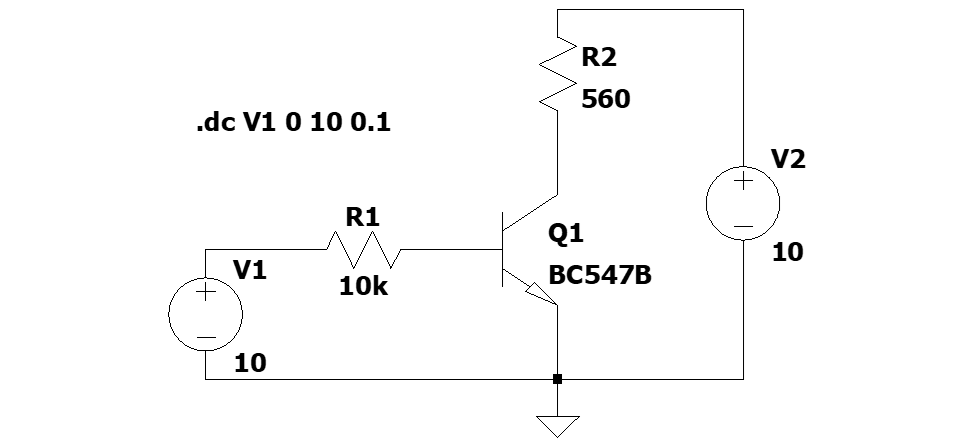
\includegraphics[width=1\textwidth, keepaspectratio]{pictures/circuito-simulacion-pol-junt-BE.png}
        \caption{Circuito polarización de juntura BE para $V_{CC} = 10V$ simulado en LTSpice}
        \label{fig:circuito-simulacion-pol-junt-BE}
    \end{figure}

    \begin{figure}[H]
        \centering
        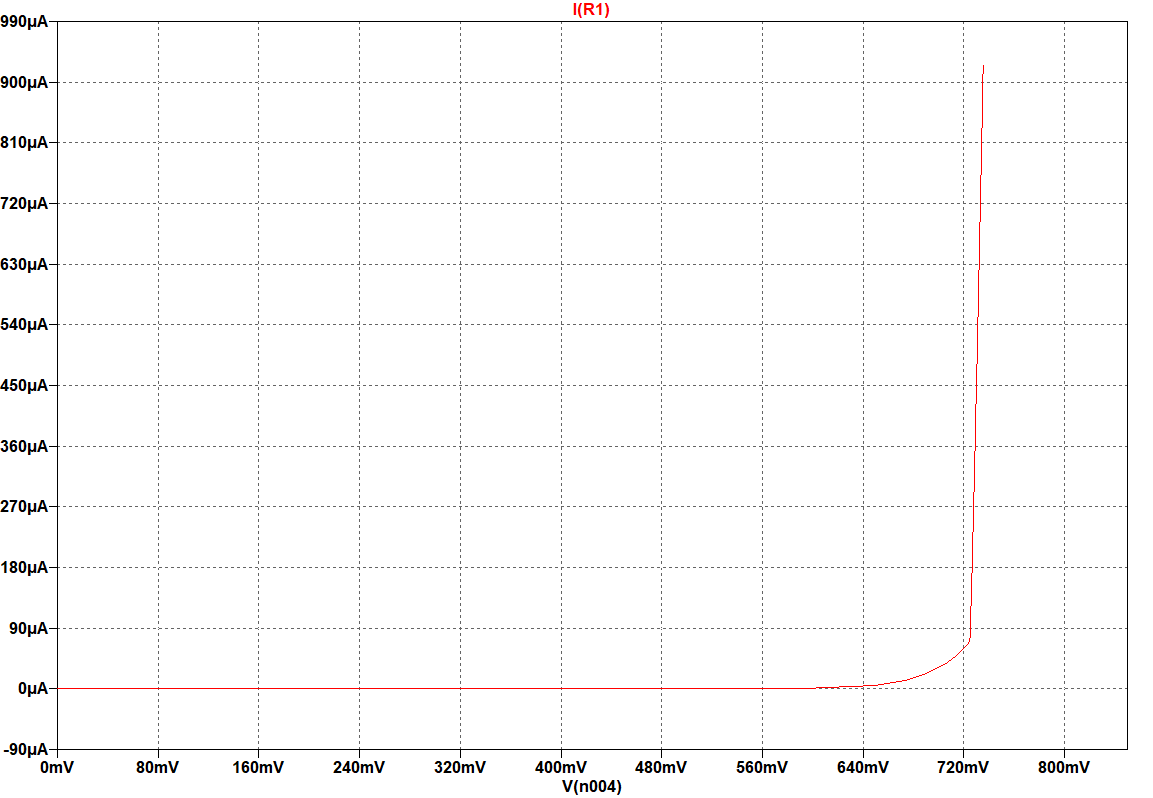
\includegraphics[width=1\textwidth, keepaspectratio]{pictures/curva-simulacion-pol-junt-be.png}
        \caption{$I_B$ en función de $V_{BE}$ resultado de simulación
        ~\ref{fig:circuito-simulacion-pol-junt-BE}}
    \end{figure}

    \begin{figure}[H]
        \centering
        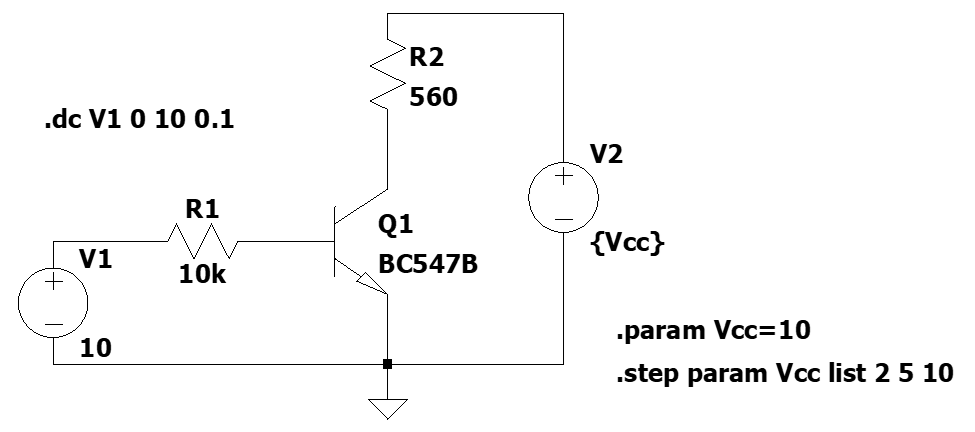
\includegraphics[width=1\textwidth, keepaspectratio]{pictures/circuito-simulacion-pol-junt-BE-variandoVCC.png}
        \caption{Circuito polarización de juntura BE variando $V_{CC}$ simulado en LTSpice}
        \label{fig:circuito-simulacion-pol-junt-BE-variandoVCC}
    \end{figure}

    \begin{figure}[H]
        \centering
        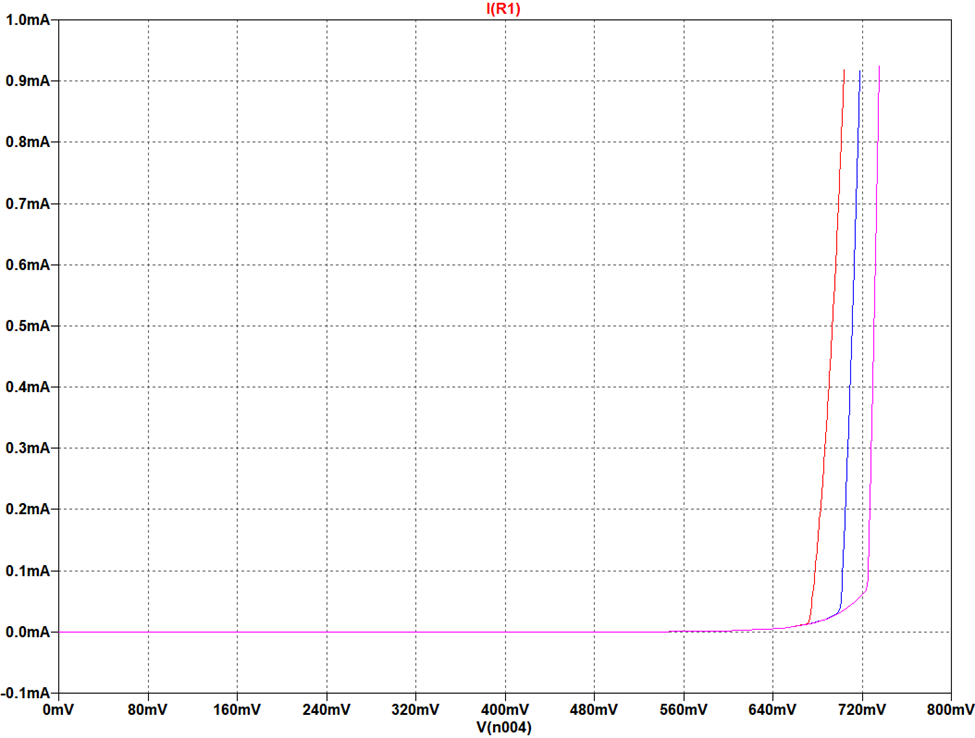
\includegraphics[width=1\textwidth, keepaspectratio]{pictures/curva-simulacion-pol-junt-be-variandoVCC.png}
        \caption{$I_B$ en función de $V_{BE}$ resultado de simulación
        ~\ref{fig:circuito-simulacion-pol-junt-BE-variandoVCC}}
    \end{figure}

    \begin{figure}[H]
        \centering
        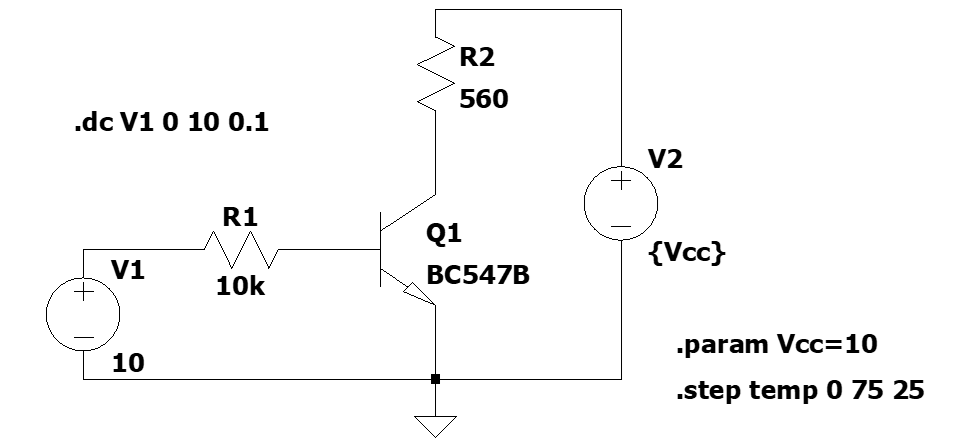
\includegraphics[width=1\textwidth, keepaspectratio]{pictures/circuito-simulacion-pol-junt-be-variandoTEMP.png}
        \caption{Circuito polarización de juntura BE variando la temperatura simulado en LTSpice}
        \label{fig:circuito-simulacion-pol-junt-BE-variandoTEMP}
    \end{figure}

    \begin{figure}[H]
        \centering
        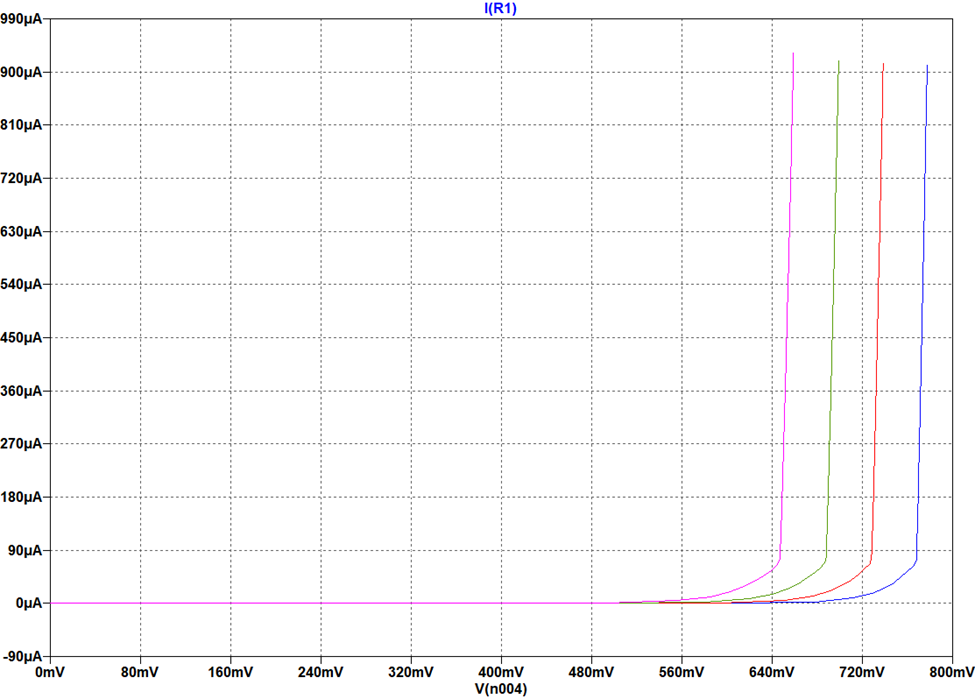
\includegraphics[width=1\textwidth, keepaspectratio]{pictures/curva-simulacion-pol-junt-be-variandoTEMP.png}
        \caption{$I_B$ en función de $V_{BE}$ resultado de simulación 
        ~\ref{fig:circuito-simulacion-pol-junt-BE-variandoTEMP}}
    \end{figure}
    
    \subsection{Actividad de laboratorio}
      \begin{center}
      \resizebox{\textwidth}{!}{%
        \begin{tabular}{|c|c|c|c|c|c|c|c|c|c|c|c|}
          \hline
          $V_{BB}$ & 0 & 0.284 V & 0.393 V & 0.5 V & 0.596 V & 0.7 V & 0.8 V & 1.06 V & 3 V & 7 V & 10 V \\
          \hline
          $I_B$ & 0 A & 29 nA & 43 nA & 91 nA & 0.78 uA & 4.99 uA & 12.46 uA & 35.84 uA & 226.3 uA & 625 uA & 929 uA \\
          \hline
          $V_{BE}$ & 0 V & 0.27 V & 0.38 V & 0.48 V & 0.57 V & 0.63 V & 0.66 V & 0.68 V & 0.73 V & 0.75 V & 0.75 V \\
          \hline
        \end{tabular}%
      }
      \end{center}

    \begin{figure}[H]
        \begin{tikzpicture}
          \begin{axis}[
            axis lines = left,
            ylabel = {$I_{B}[A]$},
            xlabel = {$V_{BE}[V]$},
            ymin=0, ymax=0.001,
            xmin=0, xmax=0.9,
            width=15cm,
            height=7cm,
            clip=false,
          ]
            \addplot[
              color=blue,
              mark=*,
              only marks,
              mark options={scale=1.3}
            ]
            coordinates {
                (0.00, 0)
                (0.27, 29e-9)
                (0.38, 43e-9)
                (0.48, 91e-9)
                (0.57, 0.78e-6)
                (0.63, 4.99e-6)
                (0.66, 12.46e-6)
                (0.68, 35.84e-6)
                (0.73, 226.3e-6)
                (0.75, 625e-6)
                (0.75, 929e-6)
            };
            \addplot[
              color=blue,
              thick
            ]
            coordinates {
                (0.00, 0)
                (0.27, 29e-9)
                (0.38, 43e-9)
                (0.48, 91e-9)
                (0.57, 0.78e-6)
                (0.63, 4.99e-6)
                (0.66, 12.46e-6)
                (0.68, 35.84e-6)
                (0.73, 226.3e-6)
                (0.75, 625e-6)
                (0.75, 929e-6)
            };
          \end{axis}
        \end{tikzpicture}
        \caption{\footnotesize $I_B$ en función de $V_{BE}$ a partir de mediciones en laboratorio}
        \end{figure}


\chapter{Curvas características}
\section{Actividad de simulación}
    \begin{figure}[H]
        \centering
        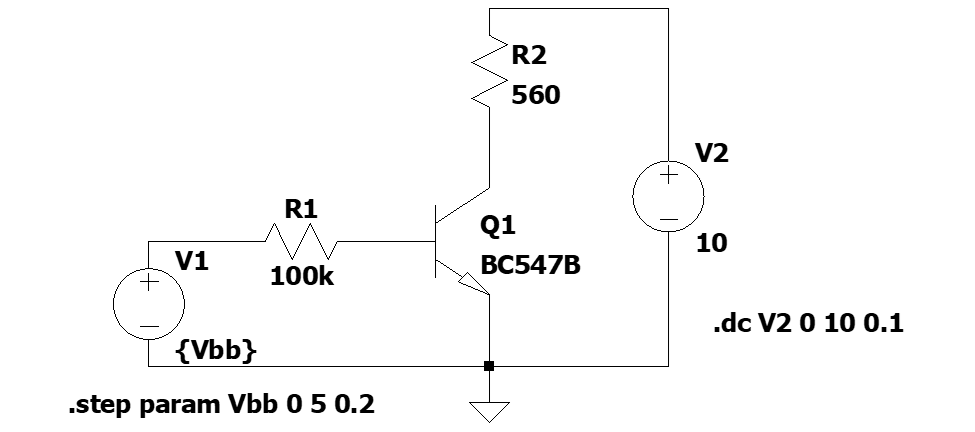
\includegraphics[width=1\textwidth, keepaspectratio]{pictures/circuito-simulacion-salida.png}
        \caption{Circuito emisor-común con fuentes variables para observar curva característica del transistor simulado en LTSpice}
        \label{fig:circuito-simulacion-salida}
    \end{figure}

    \begin{figure}[H]
        \centering
        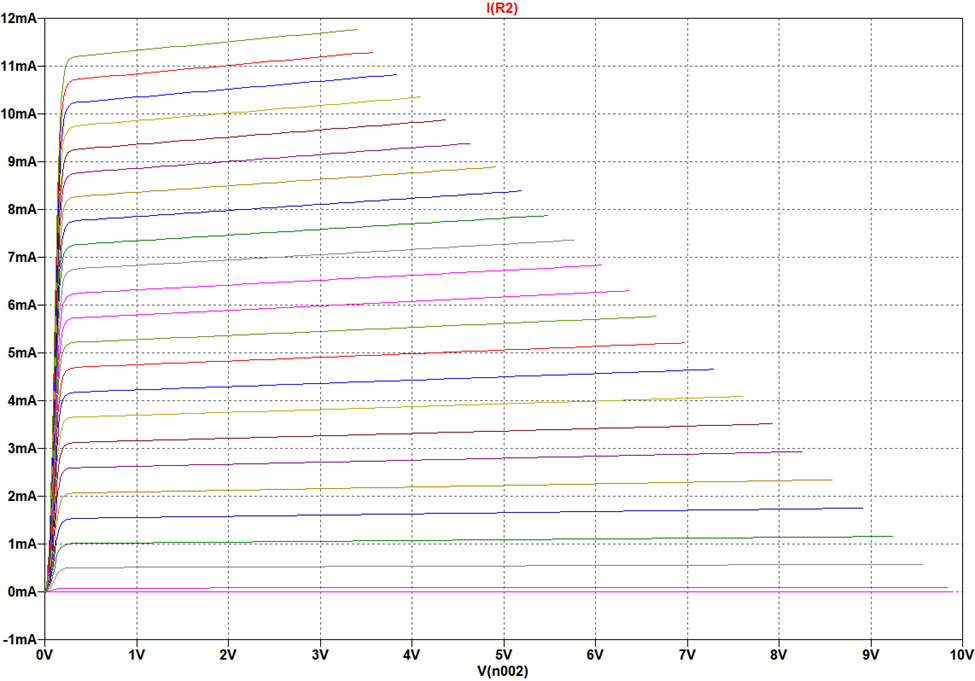
\includegraphics[width=1\textwidth, keepaspectratio]{pictures/curva-simulacion-salida.png}
        \caption{$I_C$ en función de $V_{CE}$ resultado de simulación 
        ~\ref{fig:circuito-simulacion-salida}}
    \end{figure}


\chapter{Caracteristicas de transferencia de corriente}

\chapter{Interpretacion de las especificaciones del fabricante}

\chapter{Conclusiones}


\end{document}
